% !TEX root = ../main.tex

\subsection{Spiral Winding}
\label{section:spiral_winding}
In order to test the possible progenitor distribution of our estimated galaxy pitch angles, we repeatedly perform an Anderson-Darling test over each draw present in the MCMC trace, resulting in a distribution of Anderson-Darling statistics. We will refer to this test as the \textit{marginalized Anderson-Darling test}. We make use of the Kolmogorov-Smirnov test in a similar manner for comparison.

We perform the marginalized Anderson-Darling test for a potential source distribution uniform in $\cot\phi$ between the limits present in \citet{2019arXiv190910291P} ($1.00 < \cot\phi < 4.75$, or roughly $11.9^\circ < \phi < 45.0^\circ$). The resulting distribution of Anderson-Darling statistics can be seen in Figure \ref{fig:ad-cot-test}. We observe that we reject the null hypothesis at the 1\% level for only 86\% of the possible realizations of galaxy pitch angle, therefore with our sample and methodology we cannot unilaterally reject winding of the kind described by \citet{2019arXiv190910291P}.

\begin{figure*}
  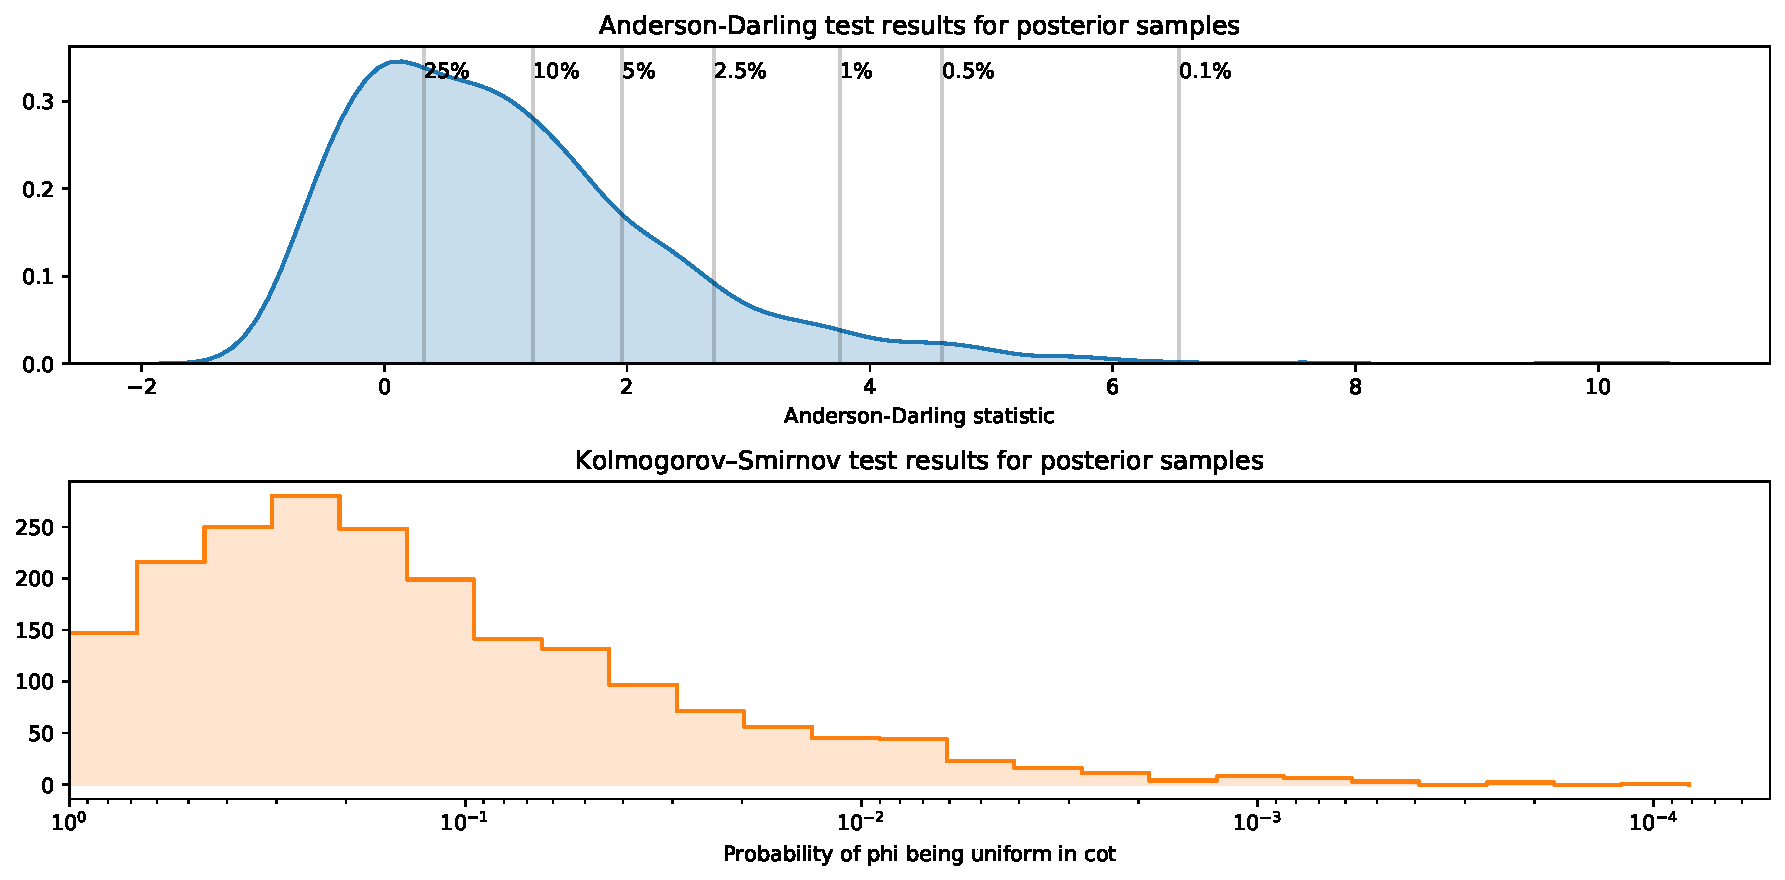
\includegraphics[width=17.7cm]{plots/cot_uniform_marginalized_tests.pdf}
  \caption{The results of a marginalized Anderson-Darling test (top panel), with confidence intervals shown, and marginalized Kolmogorov-Smirnov test p-values (lower panel). Moving rightwards on the x-axis implies greater confidence in rejecting the null hypothesis.}
  \label{fig:ad-cot-test}
\end{figure*}

\subsection{Dependence of pitch angle on Galaxy Morphology}
\label{section:morphology_comparision}
\subsubsection{Pitch angle vs. Bulge size}
We see no correlation between galaxy pitch angle derived from the \textit{hierarchial normal model} and Galaxy Zoo 2's debiased \citep{Willett2013:1308.3496v2} \textit{pbulge}, which has been shown to be a good measure of bulge size.

We separate our sample into ``disc-dominated galaxies'' and ``obvious bulge galaxies'' using the debiased fractions from Galaxy Zoo 2 following \citet{2017MNRAS.469.3363K}, defining \textit{no bulge + just noticeable $>$ obvious + dominant} for the former and the converse for the latter. A marginalized two-sample Anderson-Darling test \citep{doi:10.1080/01621459.1987.10478517} does not find strong evidence that the samples were drawn from different distributions; we reject the null hypothesis at the 1\% level for only 8\% of the samples.


\subsubsection{Pitch angle vs. Bar Strength}
We see no correlation between galaxy pitch angle derived from the \textit{hierarchial normal model} and Galaxy Zoo 2's debiased \textit{pbar}, which is widely viewed as a good measure of bar strength, and therefore a measure of the torque applied on the disc gas.

Separating the sample based off of $\mathrm{\textit{pbar}} > 0.5$, and restricting to galaxies with more than 10 classifications for \textit{pbar} (as performed by \citealt{2011MNRAS.411.2026M} and \citealt{2017MNRAS.469.3363K}) and performing a marginalized two-sample Anderson-Darling test does not find that the samples were drawn from different distributions.


\begin{figure*}
  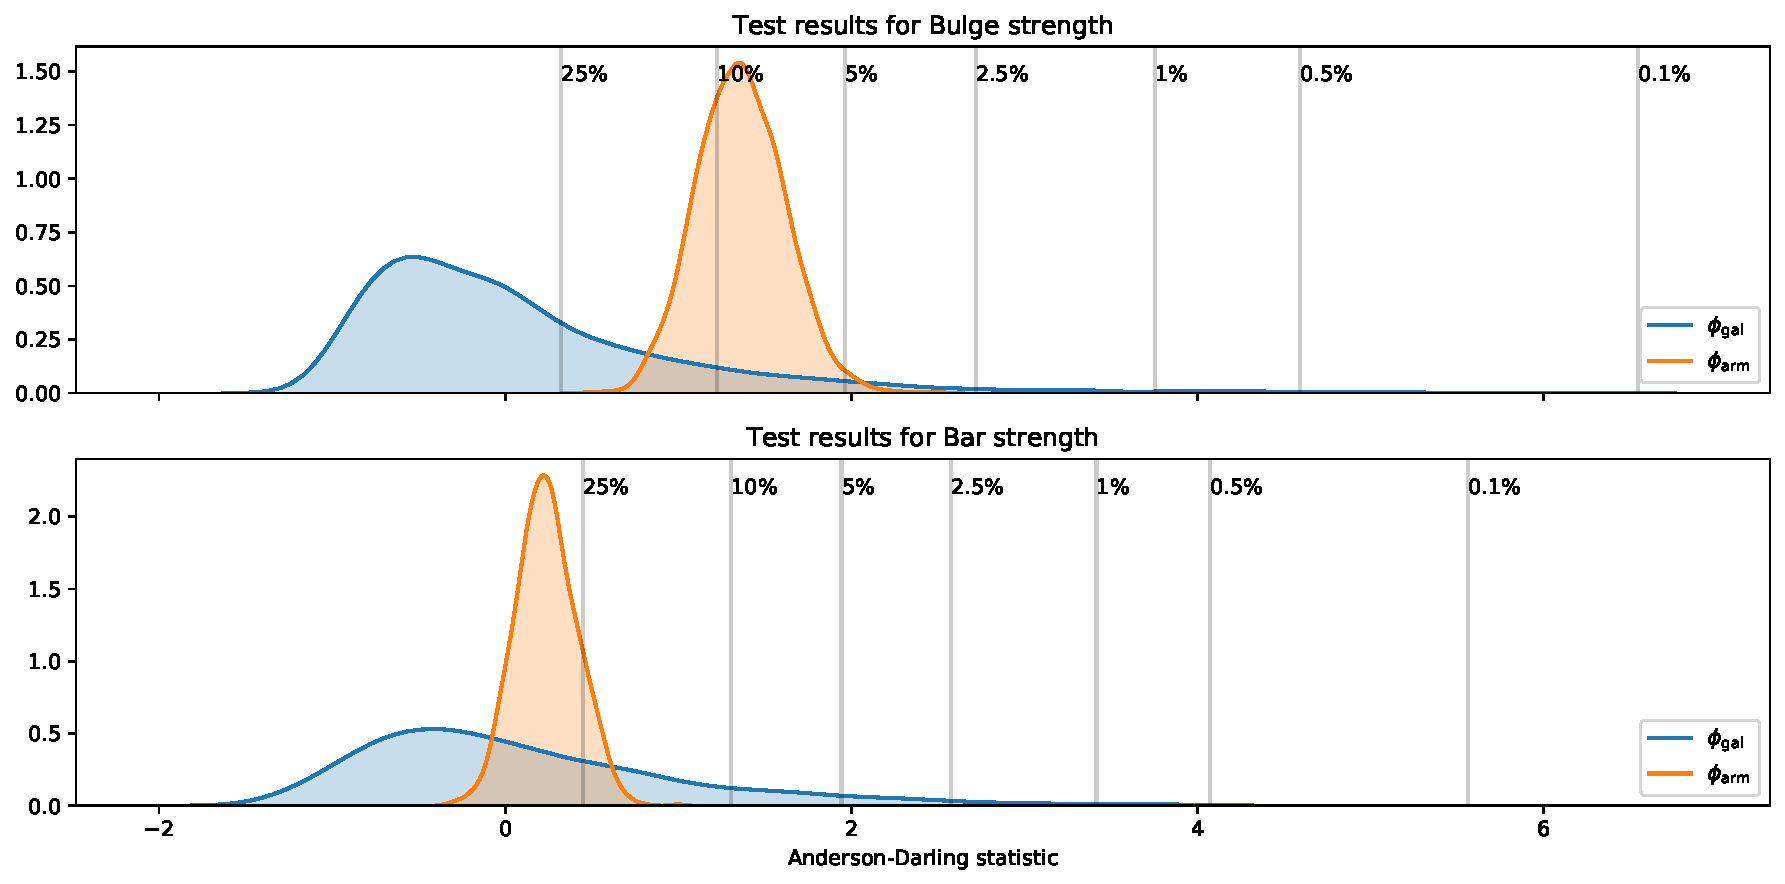
\includegraphics[width=17.7cm]{plots/bulge_bar_test_results.pdf}
  \caption{The results of marginalized two-sample Anderson-Darling tests examining whether pitch angles for Bulge-dominated and Disc-dominated galaxies are drawn from the same distribution (top panel), and the results of the same test for strongly-barred vs unbarred galaxies (bottom panel).}
  \label{fig:ad-morphology-test}
\end{figure*}
